\subsection{Şâle Köşkü ve Çit Kasrı}
\begin{wrapfigure}{r}{0.3\textwidth}
    \centering
    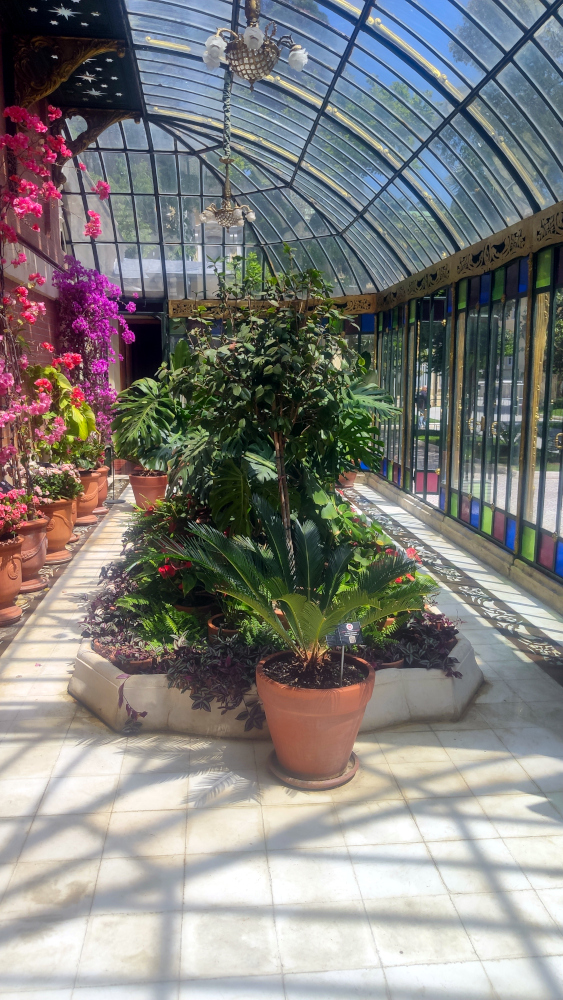
\includegraphics[width=0.25\textwidth]{assets/winter_garden.jpg}
    \caption{Çit Kasrı Kış Bahçesi}
\end{wrapfigure}
\indent\indent Yıldız Sarayı’nın dış bahçesinde yer alan Şâle Köşkü, saray kompleksine sonradan eklenen en görkemli yapılardan biridir. İmparator II. Wilhelm’in 1889 ve 1898 yıllarındaki ziyaretleri için Alexandre Vallaury ve Raimondo d’Aronco tarafından inşa edilen köşk, Batı mimarisinden etkiler taşıyan üç bölümlü yapısıyla dikkat çeker. Resmî tören ve konuk ağırlama amacıyla kullanılan Şâle Köşkü, geç dönem Osmanlı diplomasi mimarisinin simgesel yapılarındandır.\cite{dia_7}\newline
\indent Bu yapının yakınındaki Çit Kasrı, hem padişahın dinlenme köşkü hem de savaş zamanı yönetim merkezi olarak işlev kazanmış, sade fakat işlevsel mimarisiyle ön plana çıkmıştır. Her iki yapı da saray içi ve dışı alanlar arasında geçiş sağlayan, simgesel ve stratejik önem taşıyan yapılardır.\cite{dia_7}